%======================================================================
\NEWMOD
%======================================================================

\section{\sParameters}

%----------------------------------------------------------------------

\logo{\hfill\hyperlink{outline<1>}{\icon}}

\begin{frame}[fragile,label=s-parameters] 
\modframetitle{\sParameters}
\small
\begin{center}
\begin{minipage}{3.25in}
\begin{enumerate}
\item \hyperlink{ss-param-intro<1>}   {\BUTTON {\ssParamIntro}}
\item \hyperlink{ss-parameters<1>}   {\BUTTON {\ssParameters}}
\item \hyperlink{ss-doublemach<1>}     {\BUTTON {\ssDoubleMach}}
% \item \hyperlink{ss-param-problem<1>}   {\BUTTON {\ssParamProblem}}
% \item \hyperlink{ss-param-refine<1>}   {\BUTTON {\ssParamRefine}}
% \item \hyperlink{ss-param-data<1>}   {\BUTTON {\ssParamData}}
% \item \hyperlink{ss-param-method<1>}   {\BUTTON {\ssParamMethod}}
% \item \hyperlink{ss-param-io<1>}   {\BUTTON {\ssParamIo}}
% \item \hyperlink{ss-param-other<1>}   {\BUTTON {\ssParamOther}}
\item \hyperlink{ss-param-activity<1>}     {\BUTTON {\ssParamActivity}}
\item \hyperlink{ss-parameters-summary<1>}     {\BUTTON {\ssParametersSummary}}
\end{enumerate}
\end{minipage}
\end{center}
\end{frame}

\logo{\hfill\hyperlink{s-parameters<1>}{\icon}}

%======================================================================
\NEWSEC
%======================================================================

\subsection{\ssParamIntro}

\begin{frame}[fragile,label=ss-param-intro] 
\secframetitle{\ssParamIntro}
\framesubtitle{Introduction to Enzo-P/Cello parameter files}
\textbf{Enzo-P uses \textit{structured} parameter files}
\footnotesize
\pause
\begin{itemize}
\item \parameter{parameters} are organized into \group{Groups} and \subgroup{subgroups}
\pause
\begin{minipage}{3in}
\vspace{0.1in}
\begin{semiverbatim}
\group{Initial} \{
    list = ["value"];
    \subgroup{value} \{
       \parameter{velocity_x = 1.0};
   \}
\}
\end{semiverbatim}
\end{minipage}
\pause
\item parameters have a variety of types
\pause
\begin{minipage}{3in}
\vspace{0.1in}
  \begin{tabbing}
xxxxxxxxxxxxxxxxx\=xxxxxxxxxxxxxxxxxx\=\kill
\>  \uncover<5->{\textit{floating-point}:} \' \uncover<5->{\parameter{value} \texttt{=} \valuetext{1.0};} \\
\>  \uncover<6->{\textit{integers}:} \' \uncover<6->{\parameter{cycle} \texttt{=} \valuetext{100};} \\
\>  \uncover<7->{\textit{logical}:} \' \uncover<7->{\parameter{crash} \texttt{=} \valuetext{false};} \\
\>  \uncover<8->{\textit{string}:} \' \uncover<8->{\parameter{type} \texttt{=} \valuetext{"dinosaur"};} \\
\>  \uncover<9->{\textit{lists}:} \' \uncover<9->{\parameter{list} \texttt{=} \valuetext{["density", "gravity"]};} \\
\>  \uncover<10->{\textit{FP-expressions}:} \'  \uncover<10->{\parameter{value} \texttt{=} \valuetext{1.0 + 3.0*sin(x)};} \\
\>  \uncover<11->{\textit{logical-expressions}:} \' \uncover<11->{\parameter{mask} \texttt{=} \valuetext{(x >= 4.0) || (y >= 1.0)};}
\end{tabbing}
\end{minipage}
\end{itemize}
\end{frame}

%======================================================================

\begin{frame}[fragile]
\secframetitle{\ssParamIntro}
\framesubtitle{Introduction to Enzo-P/Cello parameter files}
\footnotesize
\begin{itemize}
\item Groups can be disjoint
\pause
\begin{semiverbatim}
\uncover<+->{\group{Method} \{
   \parameter{list} = \valuetext{["ppm"]};
\}}
\uncover<+->{\group{Method} \{
   \subgroup{ppm} \{
       \parameter{dual_energy} = \valuetext{true};
    \}
\}}
\end{semiverbatim}
\uncover<+->{\item Multiple parameter assignments use last value}
\begin{semiverbatim}
\uncover<+->{\parameter{list} = \valuetext{["ppm", "gravity"];}}
\uncover<+->{\parameter{list} = \valuetext{["gravity","ppm"];} \textsf{\comment{\# this value used}}}
\uncover<+->{\parameter{list} += \valuetext{["pm_update"];} \textsf{\comment{\# lists can be appended to}}}
\end{semiverbatim}
\uncover<+->{\item \comment{\# Hi! I'm a comment.}}
\end{itemize}
\end{frame}

%======================================================================



\begin{frame}[fragile] 
\secframetitle{\ssParamIntro}
\framesubtitle{Introduction to Enzo-P/Cello parameter files}

\begin{itemize}
\uncover<+->{\item Files can be \bluecode{included}}
\begin{semiverbatim}
\uncover<+->{\group{Output \{ }
   \subgroup{density} \{
      \bluecode{include} \valuetext{"input/schedule_cycle_100.incl"}
   \}
\}}
\end{semiverbatim}
\uncover<+->{\item Complicated ``including'' of files can be confusing}
\uncover<+->{\item Cello outputs a \greencode{parameters.out} file}
\begin{itemize}
\uncover<+->{\item contains all parameters}
\uncover<+->{\item organized alphabetically}
\uncover<+->{\item can be used as an input parameter file}
\end{itemize}
\end{itemize}

\end{frame}
%======================================================================


\begin{frame}[fragile]
\secframetitle{\ssParamIntro}
\framesubtitle{Parameter file issues}
% Review ss-bugs.tex / http://client64-249.sdsc.edu/cello-bug

\begin{itemize}
   \item Floats and integers cannot be mixed
   \cornersize{0.9}
   \begin{itemize}
     \item[\frownie] \textcolor{red}{\code{velocity\_x = 8.0 + 2*x }}
     \item[\smiley] \textcolor{green!50!black}{\code{velocity\_x = 8.0 + 2.0*x}}
   \end{itemize}

   \item Need space after subtraction minus sign
   \begin{itemize}
     \item[\frownie] \textcolor{red}{\code{density = x -2.0;}}
     \item[\smiley] \textcolor{green!50!black}{\code{density = x - 2.0;}}
   \end{itemize}
  \item Need at least as many root blocks as processors $P$
  \begin{itemize}
    \item \code{Mesh \{ root\_blocks = [4,4,4]; \} }
    \item[\frownie] \textcolor{red}{\code{\$ charmrun +p72} \code{bin/enzo-p \ldots}}
    \item[\smiley]\textcolor{green!50!black}{\code{\$ charmrun +p64} \code{bin/enzo-p \ldots}}
  \end{itemize}
  \item AMR requires ghost zone depth of $\ge 4$
\end{itemize}

\link{ss-bugs}{Other issues: see bug tracking website}

\end{frame}

 % Enzo-P / Cello parameter files
%======================================================================
\NEWSEC
%======================================================================

\subsection{\ssParameters}

\begin{frame}[fragile,label=ss-parameters] 
\secframetitle{\ssParameters}
\framesubtitle{Writing parameter files by \group{Group}}
\vspace{-0.2in}
\begin{minipage}[t]{1.7in}
\begin{itemize}
\item 
\textcolor{blue}{Problem definition}
  \begin{itemize}
\pause
\item
\begin{tabbing}
xxxxxxxxxxxxxxxxxxxxxxxxxx\=\kill
  \textcolor{blue}{\code{Domain}} \> \blueit{domain extents}
\end{tabbing}
\item \begin{tabbing}
xxxxxxxxxxxxxxxxxxxxxxxxxx\=\kill
  \textcolor{blue}{\code{Initial}} \> \blueit{initial conditions}
\end{tabbing}
\item \begin{tabbing}
xxxxxxxxxxxxxxxxxxxxxxxxxx\=\kill
  \textcolor{blue}{\code{Boundary}} \> \blueit{boundary conditions}
\end{tabbing}
\pause
  \item \begin{tabbing}
xxxxxxxxxxxxxxxxxxxxxxxxxx\=\kill
 \textcolor{blue}{\code{Stopping}} \> \blueit{stopping criteria}
\end{tabbing}
  \end{itemize}
\pause
\item \textcolor{green!50!black}{Discretization}
  \begin{itemize}
  \item \begin{tabbing}
xxxxxxxxxxxxxxxxxxxxxxxxxx\=\kill
 \textcolor{green!50!black}{\code{Mesh}} \> \greenit{root mesh blocking}
  \end{tabbing}  
  \item \begin{tabbing}
xxxxxxxxxxxxxxxxxxxxxxxxxx\=\kill
 \textcolor{green!50!black}{\code{Adapt}} \> \greenit{adaptive mesh refinement}
   \end{tabbing}
\pause
  \item \begin{tabbing}
xxxxxxxxxxxxxxxxxxxxxxxxxx\=\kill
 \textcolor{green!50!black}{\code{Field}} \> \greenit{field data}
   \end{tabbing}
  \end{itemize}
\pause
\item \textcolor{red!50!black}{Parallel computation}
  \begin{itemize}
\pause
  \item \begin{tabbing}
xxxxxxxxxxxxxxxxxxxxxxxxxx\=\kill
 \textcolor{red!50!black}{\code{Method}} \> \redit{computational methods}
  \end{tabbing}
  \end{itemize}
\pause
\item \textcolor{cyan!50!black}{Output}
  \begin{itemize}
\pause
    \item \begin{tabbing}
xxxxxxxxxxxxxxxxxxxxxxxxxx\=\kill
 \textcolor{cyan!50!black}{\code{Output}} \> \cyanit{disk output}
    \end{tabbing}
  \end{itemize}
\end{itemize}
\end{minipage}
\end{frame}

%======================================================================
% \secframetitle{\ssParameters}
% \framesubtitle{\ }
% \begin{minipage}[t]{1.7in}
% \begin{itemize}
% \item \textcolor{blue}{Problem definition}
%   \begin{itemize}
%   \item \textcolor{blue}{\code{Domain}}
%   \item \textcolor{blue}{\code{Initial}}
%   \item \textcolor{blue}{\code{Boundary}}
%   \item \textcolor{blue}{\code{Stopping}}
%   \end{itemize}
% \item \textcolor<1>{green!50!black}{Discretization}
%   \begin{itemize}
%   \item \textcolor<1>{green!50!black}{\code{Mesh}}
%   \item \textcolor<1>{green!50!black}{\code{Adapt}}
%   \item \textcolor<1>{green!50!black}{\code{Field}}
%   \end{itemize}
% \item \textcolor<1>{red!50!black}{Parallel computation}
%   \begin{itemize}
%   \item \textcolor<1>{red!50!black}{\code{Method}}
%   \end{itemize}
% \item \textcolor<1>{cyan!50!black}{Output}
%   \begin{itemize}
%     \item \textcolor<1>{cyan!50!black}{\code{Output}}
%   \end{itemize}
% \end{itemize}
% \end{minipage}
% \end{frame}

%----------------------------------------------------------------------

\begin{frame}[fragile] 
\secframetitle{\ssParameters}
\framesubtitle{Problem parameters}
\vspace{-0.2in}
\begin{minipage}[t]{1.7in}
\begin{itemize}
\item \bfat{1}{\textcolor{blue}{Problem definition}}
  \begin{itemize}
  \item \bfat{1}{\textcolor{blue}{\code{Domain}}}
  \item \textcolor{blue}{\code{Initial}}
  \item \textcolor{blue}{\code{Boundary}}
  \item \textcolor{blue}{\code{Stopping}}
  \end{itemize}
\item Discretization
  \begin{itemize}
  \item \code{Mesh}
  \item \code{Adapt}
  \item \code{Field}
  \end{itemize}
\item Parallel computation
  \begin{itemize}
  \item \code{Method}
  \end{itemize}
\item Output
  \begin{itemize}
    \item \code{Output}
  \end{itemize}
\end{itemize}
\end{minipage} \
%- - - - - - - - - - - - - - - - - - -
\begin{minipage}[t]{2.6in}
\vspace{-0.2in}
\setbeamercolor{block title}{bg=blue!30,fg=black}
\begin{block}{\textbf{Domain definition}}
\footnotesize \vspace{-0.1in}
\begin{semiverbatim}
\group{Domain} \{
   \variable{lower} = [\valuetext{0.0}, \valuetext{0.0}];
   \variable{upper} = [\valuetext{0.3}, \valuetext{0.3}];
\} 
\end{semiverbatim}
\end{block}
\end{minipage}
\end{frame}


%----------------------------------------------------------------------

\begin{frame}[fragile] 
\secframetitle{\ssParameters}
\framesubtitle{Problem parameters}
\vspace{-0.2in}
\begin{minipage}[t]{1.7in}
\begin{itemize}
\item \bfat{1}{\textcolor{blue}{Problem definition}}
  \begin{itemize}
  \item \textcolor{blue}{\code{Domain}}
  \item \bfat{1}{\textcolor{blue}{\code{Initial}}}
  \item \textcolor{blue}{\code{Boundary}}
  \item \textcolor{blue}{\code{Stopping}}
  \end{itemize}
\item Discretization
  \begin{itemize}
  \item \code{Mesh}
  \item \code{Adapt}
  \item \code{Field}
  \end{itemize}
\item Parallel computation
  \begin{itemize}
  \item \code{Method}
  \end{itemize}
\item Output
  \begin{itemize}
    \item \code{Output}
  \end{itemize}
\end{itemize}
\end{minipage} \
%- - - - - - - - - - - - - - - - - - -
\begin{minipage}[t]{2.6in}
\vspace{-0.2in}
\setbeamercolor{block title}{bg=blue!30,fg=black}
\begin{block}{\textbf{Initial Conditions}}
\footnotesize \vspace{-0.1in}
\begin{semiverbatim}
\group{Initial} \{
   \variable{type} = \valuetext{"value"};
   \subgroup{density} \{
      \variable{value} = [ \valuetext{0.125},   \variable{x} +  \variable{y} <  \valuetext{0.15}, 
                \valuetext{1.0} ];
   \};
   \subgroup{total_energy} \{
        \variable{value} = [  \valuetext{0.14} / ( \valuetext{0.4} *  \valuetext{0.125}),
                     \variable{x} +  \variable{y} <  \valuetext{0.15},
                  \valuetext{1.00} / ( \valuetext{0.4} *  \valuetext{1.000}) ];
   \};
\}
\end{semiverbatim}
\end{block}
\end{minipage}
\end{frame}

\begin{frame}[fragile] 
\secframetitle{\ssParameters}
\framesubtitle{Problem parameters}
\vspace{-0.2in}
\begin{minipage}[t]{1.7in}
\begin{itemize}
\item \bfat{1}{\textcolor{blue}{Problem definition}}
  \begin{itemize}
  \item \textcolor{blue}{\code{Domain}}
  \item \textcolor{blue}{\code{Initial}}
  \item \bfat{1}{\textcolor{blue}{\code{Boundary}}}
  \item \bfat{2}{\textcolor{blue}{\code{Stopping}}}
  \end{itemize}
\item Discretization
  \begin{itemize}
  \item \code{Mesh}
  \item \code{Adapt}
  \item \code{Field}
  \end{itemize}
\item Parallel computation
  \begin{itemize}
  \item \code{Method}
  \end{itemize}
\item Output
  \begin{itemize}
    \item \code{Output}
  \end{itemize}
\end{itemize}
\end{minipage} \
%- - - - - - - - - - - - - - - - - - -
\begin{minipage}[t]{2.6in}
\vspace{-0.2in}
\setbeamercolor{block title}{bg=blue!30,fg=black}
 \begin{block}<+->{\textbf{Boundary conditions}}
 \footnotesize \vspace{-0.1in}
 \begin{semiverbatim}
\group{Boundary} \{
   \variable{list} = [\valuetext{"x_bc"}, \valuetext{"y_bc"}];
   \subgroup{x_bc} \{ \variable{axis} = \valuetext{"x"}; \variable{type} = \valuetext{"reflecting"}; \};
   \subgroup{y_bc} \{ \variable{axis} = \valuetext{"y"}; \variable{type} = \valuetext{"periodic"}; \};
\}
 \end{semiverbatim}
 \end{block}
 \begin{block}<+->{\textbf{Stopping criteria}}
 \footnotesize \vspace{-0.1in}
 \begin{semiverbatim}
 \group{Stopping} \{ \variable{cycle} = \valuetext{100}; \}
 \end{semiverbatim}
 \end{block}
\end{minipage}
\end{frame}

%----------------------------------------------------------------------

\begin{frame}[fragile] 
\secframetitle{\ssParameters}
\framesubtitle{Discretization parameters}
\vspace{-0.2in}
\begin{minipage}[t]{1.7in}
\begin{itemize}
\item Problem definition
  \begin{itemize}
  \item \code{Domain}
  \item \code{Initial}
  \item \code{Boundary}
  \item \code{Stopping}
  \end{itemize}
\item \bfat{1-2}{\textcolor{green!50!black}{Discretization}}
  \begin{itemize}
  \item \bfat{1}{\textcolor{green!50!black}{\code{Mesh}}}
  \item \bfat{2}{\textcolor{green!50!black}{\code{Adapt}}}
  \item \textcolor{green!50!black}{\code{Field}}
  \end{itemize}
\item Parallel computation
  \begin{itemize}
  \item \code{Method}
  \end{itemize}
\item Output
  \begin{itemize}
    \item \code{Output}
  \end{itemize}
\end{itemize}
\end{minipage} \
%- - - - - - - - - - - - - - - - - - -
\begin{minipage}[t]{2.6in}
\vspace{-0.2in}
\setbeamercolor{block title}{bg=green!30,fg=black}
\begin{block}<+->{\textbf{Mesh hierarchy control}}
  \footnotesize \vspace{-0.1in}
\begin{semiverbatim}
\group{Mesh} \{ 
   \variable{root_rank}   = \valuetext{2};
   \variable{root_size}   = [\valuetext{400},\valuetext{400}];
   \variable{root_blocks} = [\valuetext{4},\valuetext{4}];
\}
\end{semiverbatim}
\begin{semiverbatim}
\uncover<2->{\group{Adapt} \{
   \variable{max_level} = \valuetext{5};
   \variable{list} = [\valuetext{"SLOPE"}];
   \subgroup{SLOPE} \{
      \variable{type} = \valuetext{"slope"};
      \variable{field_list} = [\valuetext{"density"}];
   \}
\}
}
\end{semiverbatim}
\end{block}
\end{minipage}
\end{frame}

%----------------------------------------------------------------------

\begin{frame}[fragile] 
\secframetitle{\ssParameters}
\framesubtitle{Discretization parameters}
\vspace{-0.2in}
\begin{minipage}[t]{1.7in}
\begin{itemize}
\item Problem definition
  \begin{itemize}
  \item \code{Domain}
  \item \code{Initial}
  \item \code{Boundary}
  \item \code{Stopping}
  \end{itemize}
\item \bfat{1}{\textcolor{green!50!black}{Discretization}}
  \begin{itemize}
  \item \textcolor{green!50!black}{\code{Mesh}}
  \item \textcolor{green!50!black}{\code{Adapt}}
  \item \bfat{1}{\textcolor{green!50!black}{\code{Field}}}
  \end{itemize}
\item Parallel computation
  \begin{itemize}
  \item \code{Method}
  \end{itemize}
\item Output
  \begin{itemize}
    \item \code{Output}
  \end{itemize}
\end{itemize}
\end{minipage} \
%- - - - - - - - - - - - - - - - - - -
\begin{minipage}[t]{2.6in}
\vspace{-0.2in}
\setbeamercolor{block title}{bg=green!30,fg=black}
  \begin{block}<+->{\textbf{Field variables}}
  \footnotesize \vspace{-0.1in}
\begin{semiverbatim}
\group{Field} \{
   \variable{list} = [\valuetext{"density"},
           \valuetext{"velocity_x"},
           \valuetext{"velocity_y"},
           \valuetext{"total_energy"},
           \valuetext{"pressure"}];
   \variable{courant}   = \valuetext{0.8};
   \variable{ghosts}    = \valuetext{3};
   \variable{alignment} = \valuetext{8};    
\}
\end{semiverbatim}
\end{block}
\end{minipage}
\end{frame}
  

%----------------------------------------------------------------------

\begin{frame}[fragile] 
\secframetitle{\ssParameters}
 \framesubtitle{Parallel computation parameters}
\vspace{-0.2in}
\begin{minipage}[t]{1.80in}
\begin{itemize}
\item Problem definition
  \begin{itemize}
  \item \code{Domain}
  \item \code{Initial}
  \item \code{Boundary}
  \item \code{Stopping}
  \end{itemize}
\item Discretization
  \begin{itemize}
  \item \code{Mesh}
  \item \code{Adapt}
  \item \code{Field}
  \end{itemize}
\item \bfat{1}{\textcolor{red!50!black}{Parallel computation}}
  \begin{itemize}
  \item \bfat{1}{\textcolor{red!50!black}{\code{Method}}}
  \end{itemize}
\item Output
  \begin{itemize}
    \item \code{Output}
  \end{itemize}
\end{itemize}
\end{minipage} \
%- - - - - - - - - - - - - - - - - - -
%- - - - - - - - - - - - - - - - - - -
\begin{minipage}[t]{2.50in}
\vspace{-0.2in}
\setbeamercolor{block title}{bg=red!30,fg=black}
 \begin{block}<+->{\textbf{Method list}}
 \footnotesize \vspace{-0.1in}
\begin{semiverbatim}
\group{Method} \{
   \variable{list} = [\valuetext{"ppm"},\valuetext{"gravity_bicgstab"}];
   \subgroup{ppm} \{
      \variable{diffusion}   = \valuetext{true};
      \variable{steepening}  = \valuetext{true};
   \};
   \subgroup{gravity_bicgstab} \{
      \variable{iter_max} = \valuetext{100};
      \variable{res_tol}  = \valuetext{0.001};
   \}
\}
\end{semiverbatim}
\end{block}
\end{minipage}
\end{frame}

%----------------------------------------------------------------------

% \begin{frame}[fragile] 
% \secframetitle{\ssParameters}
%  \framesubtitle{Parallel computation parameters}
% \vspace{-0.2in}
% \begin{minipage}[t]{1.80in}
% \begin{itemize}
% \item Problem definition
%   \begin{itemize}
%   \item \code{Domain}
%   \item \code{Initial}
%   \item \code{Boundary}
%   \item \code{Stopping}
%   \end{itemize}
% \item Discretization
%   \begin{itemize}
%   \item \code{Mesh}
%   \item \code{Adapt}
%   \item \code{Field}
%   \end{itemize}
% \item \bfat{1}{\textcolor{red!50!black}{Parallel computation}}
%   \begin{itemize}
%   \item \code{Method}
%   \end{itemize}
% \item Output
%   \begin{itemize}
%     \item \code{Output}
%   \end{itemize}
% \end{itemize}
% \end{minipage} \
%- - - - - - - - - - - - - - - - - - -
%- - - - - - - - - - - - - - - - - - -
% \begin{minipage}[t]{2.50in}
% \vspace{-0.2in}
% \setbeamercolor{block title}{bg=red!30,fg=black}
%  \begin{block}<+->{\textbf{Refresh list}}
%  \footnotesize \vspace{-0.1in}
% \begin{verbatim}
% Refresh {
%    list = ["ppm_refresh"];
%    ppm_refresh { 
%       field_face_rank = 0;
%       field_ghosts = 4;
%    }
% }
% \end{verbatim}
% \end{block}
% \end{minipage}
% \end{frame}

%----------------------------------------------------------------------

\begin{frame}[fragile] 
\secframetitle{\ssParameters}
\framesubtitle{Output parameters}
\vspace{-0.2in}
\begin{minipage}[t]{1.7in}
\begin{itemize}
\item Problem definition
  \begin{itemize}
  \item \code{Domain}
  \item \code{Initial}
  \item \code{Boundary}
  \item \code{Stopping}
  \end{itemize}
\item Discretization
  \begin{itemize}
  \item \code{Mesh}
  \item \code{Adapt}
  \item \code{Field}
  \end{itemize}
\item Parallel computation
  \begin{itemize}
  \item \code{Method}
  \end{itemize}
\item \bfat{1}{\textcolor{cyan!50!black}{Output}}
  \begin{itemize}
    \item \bfat{1}{\textcolor{cyan!50!black}{\code{Output}}}
  \end{itemize}
\end{itemize}
\end{minipage} \
%- - - - - - - - - - - - - - - - - - -
%- - - - - - - - - - - - - - - - - - -
\begin{minipage}[t]{2.6in}
\vspace{-0.2in}
\setbeamercolor{block title}{bg=cyan!50,fg=black}
 \begin{block}<+->{\textbf{Output files}}
 \footnotesize \vspace{-0.1in}
\begin{semiverbatim}
\group{Output} \{
   \variable{list} = [ \valuetext{"de_hdf5"}, \valuetext{"de_png"} ];
   \subgroup{de_hdf5} \{
      \comment{\# HDF5 data file group}
   \};
   \subgroup{de_png} \{
      \comment{\# PNG image file group}
   \}
\}
\end{semiverbatim}
 \end{block}
 \end{minipage}
\end{frame}
 
%----------------------------------------------------------------------
 
\begin{frame}[fragile] 
\secframetitle{\ssParameters}
\framesubtitle{Output parameters}
\vspace{-0.2in}
\begin{minipage}[t]{1.7in}
\begin{itemize}
\item Problem definition
  \begin{itemize}
  \item \code{Domain}
  \item \code{Initial}
  \item \code{Boundary}
  \item \code{Stopping}
  \end{itemize}
\item Discretization
  \begin{itemize}
  \item \code{Mesh}
  \item \code{Adapt}
  \item \code{Field}
  \end{itemize}
\item Parallel computation
  \begin{itemize}
  \item \code{Method}
  \end{itemize}
\item \bfat{1}{\textcolor{cyan!50!black}{Output}}
  \begin{itemize}
    \item \bfat{1}{\textcolor{cyan!50!black}{\code{Output}}}
  \end{itemize}
\end{itemize}
\end{minipage} \
%- - - - - - - - - - - - - - - - - - -
%- - - - - - - - - - - - - - - - - - -
\begin{minipage}[t]{2.6in}
\vspace{-0.2in}
\setbeamercolor{block title}{bg=cyan!50,fg=black}
 \begin{block}<+->{\textbf{Output files}}
 \footnotesize \vspace{-0.1in}
\begin{semiverbatim}
\group{Output} \{
   \subgroup{de_hdf5} \{
      \variable{type} = \valuetext{"data"};
      \variable{name} = [\valuetext{"implosion-%5.2f.png"},
              \valuetext{"time"}];
      \variable{field_list} = [\valuetext{"density"}];
      \subgroup{schedule} \{
         \variable{var}  = \valuetext{"time"};
         \variable{step} = \valuetext{0.02};
      \}
   \}
\}
\end{semiverbatim}
\end{block}
\end{minipage}
\end{frame}

%----------------------------------------------------------------------
 
\begin{frame}[fragile] 
\secframetitle{\ssParameters}
\framesubtitle{Output parameters}
\vspace{-0.2in}
\begin{minipage}[t]{1.7in}
\begin{itemize}
\item Problem definition
  \begin{itemize}
  \item \code{Domain}
  \item \code{Initial}
  \item \code{Boundary}
  \item \code{Stopping}
  \end{itemize}
\item Discretization
  \begin{itemize}
  \item \code{Mesh}
  \item \code{Adapt}
  \item \code{Field}
  \end{itemize}
\item Parallel computation
  \begin{itemize}
  \item \code{Method}
  \end{itemize}
\item \bfat{1}{\textcolor{cyan!50!black}{Output}}
  \begin{itemize}
    \item \bfat{1}{\textcolor{cyan!50!black}{\code{Output}}}
  \end{itemize}
\end{itemize}
\end{minipage} \
%- - - - - - - - - - - - - - - - - - -
%- - - - - - - - - - - - - - - - - - -
\begin{minipage}[t]{2.6in}
\vspace{-0.2in}
\setbeamercolor{block title}{bg=cyan!50,fg=black}
 \begin{block}<+->{\textbf{Output files}}
 \footnotesize \vspace{-0.1in}
 \begin{semiverbatim}
\group{Output} \{
   \subgroup{de_png} \{
      \variable{type} = \valuetext{"image"};
      \variable{name} = [ \valuetext{"implosion-%05d.png"},
               \valuetext{"cycle"} ];
      \variable{image_type} = \valuetext{"data"};
      \variable{colormap} = [\valuetext{0.0},\valuetext{0.0},\valuetext{0.0},
                  \valuetext{1.0},\valuetext{1.0},\valuetext{1.0}];
      \variable{field_list} = [ \valuetext{"density"} ];
      \subgroup{schedule} \{
         \variable{var} = \valuetext{"cycle"};
         \variable{step} = \valuetext{10};
      \}
   \}
\}
\end{semiverbatim}
 \end{block}
 \end{minipage}
\end{frame}

 % How do I write an Enzo-P parameter file?
%======================================================================
\NEWSEC
%======================================================================

\subsection{\ssDoubleMach}

\begin{frame}[fragile,label=ss-doublemach] 
\secframetitle{\ssDoubleMach}
\framesubtitle{Test problem specification}

\footnotesize
\begin{center}

\includegraphics[width=4.0in]{Images/DoubleMachAmr/doublemach-de-0000.png}
\end{center}

\begin{tabbing}
xxxxxxxxxxxxxxxxxxxxxxxxxxxxxxxx\=xxxxxxxxxxxxxxxxxxx\=\kill
\> \bluetext{Adiabatic index}: \' $\gamma = 1.4$. \\
\> \bluetext{Grid domain}: \' $0.0 < x < 4.0$, $0.0 < y < 1.0$ \\
\> \bluetext{Shock}: \' Mach 10, $v_s$ = 10.0, \\
\> \bluetext{Angle}: \' 30 degrees. \\
\> \bluetext{Pre-shock conditions}: \' $P = 1.0$, $\rho = 1.4$, $v = 0.0$ \\
\> \bluetext{Post-shock conditions}: \' $P = 116.5$, $\rho = 8$, $v = 8.25$ \\
\> \bluetext{Time limit}: \' $t = 0.25$.
\end{tabbing}
\end{frame}

%----------------------------------------------------------------------

\begin{frame}[fragile] 
\secframetitle{\ssDoubleMach}
\framesubtitle{\group{Domain} and \group{Stopping} criteria}
\begin{itemize}
\item \group{Domain}

\begin{itemize}
\item $0.0 < x < 4.0, 0.0 < y < 1.0$
\begin{semiverbatim}
\group{Domain} \{ 
   \parameter{lower} = [\valuetext{0.0}, \valuetext{0.0}];
   \parameter{upper} = [\valuetext{4.0}, \valuetext{1.0}];
\} 
\end{semiverbatim}
\end{itemize}
%
\item \group{Stopping} criteria
\begin{itemize}
%
\item $t=0.25$
%
\begin{semiverbatim}
\group{Stopping} \{ \variable{time} = \valuetext{0.25}; \} 
\end{semiverbatim}
%
\end{itemize}
\end{itemize}
\end{frame}

%----------------------------------------------------------------------

 \begin{frame}[fragile] 
 \secframetitle{\ssDoubleMach}
 \framesubtitle{\group{Initial} conditions}
\footnotesize
Complex initial conditions can be specified directly.

 \begin{itemize}
 \item To specify $x = a(x,y,z)$ in subregion $A$, else $x = b(x,y,z)$:
 \begin{tabbing}
 xxxxxxx\=\kill
\parameter{x} = \code{[} \> \valuetext{a(x,y,z)} \comment{\# (floating-point expression)}, \\
\>                         \valuetext{A(x,y,z)} \comment{\# (logical expression)}, \\
\>                         \valuetext{b(x,y,z)} \comment{\# (floating-point expression)} ];
 \end{tabbing}
 \item E.g. to specify ``$\rho = 8$ if $x \le 1/6 + 0.57735 y$, else $\rho = 1.4$'':
\begin{semiverbatim}
\group{Initial} \{
    \subgroup{density} \{
        \parameter{value} = [\valuetext{8.0}, \valuetext{(x <= 0.16667 + 0.57735*y)}, 
                 \valuetext{1.4}];  \};
\}
\end{semiverbatim}
\item Repeat with \subgroup{velocity\_x}, \subgroup{velocity\_y}, \subgroup{total\_energy}
 \end{itemize}
\end{frame}

%----------------------------------------------------------------------

\begin{frame}[fragile] 
\secframetitle{\ssDoubleMach}
\framesubtitle{\group{Initial} conditions}
\footnotesize
\begin{itemize}
\item Repeat with \subgroup{velocity\_x}, \subgroup{velocity\_y}, and \subgroup{total\_energy}
\begin{semiverbatim}
\group{Initial} \{
    \subgroup{velocity_x} \{
       \parameter{value} = [ \valuetext{8.25*0.8660253},
                        \valuetext{(x <= 0.16667 + 0.57735*y)},
                 \valuetext{0.0} ]; \};
    \subgroup{velocity_y} \{
       \parameter{value} = [\valuetext{-8.25*0.5},
                        \valuetext{(x <= 0.16667 + 0.57735*y)},
                 \valuetext{0.0}]; \};
    \subgroup{total_energy} \{
       \parameter{value} = [\valuetext{116.5 / (0.4 * 8.0) + 34.03125},
                        \valuetext{(x <= 0.16667 + 0.57735*y)}, 
                  \valuetext{1.0 / (0.4 * 1.4)}]; \};
 \}
\end{semiverbatim}
\end{itemize}
\end{frame}

%----------------------------------------------------------------------

 \begin{frame}[fragile] 
 \secframetitle{\ssDoubleMach}
 \framesubtitle{\group{Boundary} conditions}
\footnotesize
Complex boundary conditions can also be specified directly.

\begin{itemize}
\item General form:
 \begin{tabbing}
xxx\=xxx\=\kill
\group{Boundary} \{ \\
\>   \parameter{list} = [ \valuetext{"bc\_1"}, \valuetext{"bc\_2"}, \valuetext{"bc\_3"}, ... ];  \\
\\
\>   \subgroup{bc\_1} \{ \\
\>\>      \parameter{type} = \textit{\{} \valuetext{"inflow"}, \valuetext{"periodic"}, \valuetext{"outflow"}, \valuetext{"reflecting"} \textit{\}} \\
\>\>      \parameter{mask} = \valuetext{M(x,y,z,t)}; \comment{\# (logical expression)} \\
\>\>      \parameter{axis} = \textit{\{} \valuetext{"x"}, \valuetext{"y"}, \valuetext{"z"} \textit{\}} \\
\>\>      \parameter{face} = \textit{\{} \valuetext{"lower"}, \valuetext{"upper"}  \textit{\}} \\
\>\>      \parameter{field\_list} = [ \valuetext{velocity\_x} ]; \\
\>\>      \parameter{value} = \valuetext{M(x,y,z,t)}; \comment{\# (floating-point expression, inflow only)} \\
\>   \}; \\
\>   \subgroup{bc\_2} \{ \ldots \} \\
\}
\end{tabbing}
\end{itemize}
\end{frame}
%  
%  % 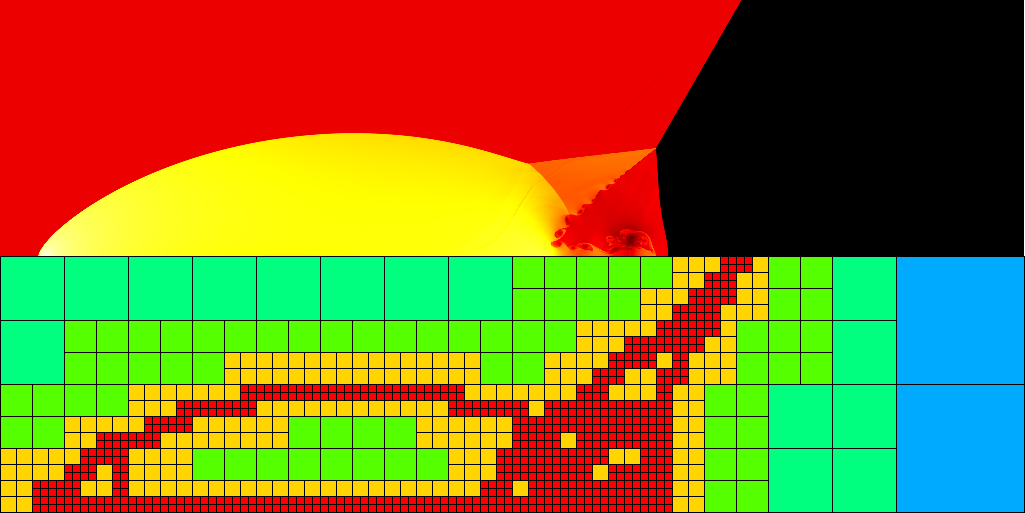
\includegraphics[width=4.0in]{Images/DoubleMachAmr/doublemach-0200.png}
%  % \ANIMATEGRAPHICS{width=4.5in}{20}{Images/DoubleMachAmr/doublemach-}{0000}{0307}
%  
%  
%  %    Boundary
%  %----------------------------------------------------------------------
%  
 \begin{frame}[fragile] 
 \secframetitle{\ssDoubleMach}
 \framesubtitle{\group{Boundary} conditions}
\footnotesize
\begin{semiverbatim}
 \group{Boundary} \{
    \variable{list} = [
            \valuetext{"OUT"},
            \valuetext{"REFLECT"},
            \valuetext{"DENSITY"},
            \valuetext{"VELOCITY_X"},
            \valuetext{"VELOCITY_Y"},
            \valuetext{"TOTAL_ENERGY}"
          ];
\}
\end{semiverbatim}
\end{frame}

%----------------------------------------------------------------------

 \begin{frame}[fragile] 
 \secframetitle{\ssDoubleMach}
 \framesubtitle{\group{Boundary} conditions: outflow and reflecting}
\footnotesize
\begin{semiverbatim}
 \group{Boundary} \{
    \subgroup{OUT} \{
       \variable{type} = \valuetext{"outflow"};
       \variable{mask} = [ (\variable{x} >= \valuetext{4.0}) || 
                (\variable{y} >= \valuetext{1.0} && (\variable{x} >= \valuetext{0.744017} + \valuetext{11.547}* \variable{t}))];
    \};
    \subgroup{REFLECT} \{
       \variable{type} = \valuetext{"reflecting"};
       \variable{axis} = \valuetext{"y"};
       \variable{face} = \valuetext{"lower"};
       \variable{mask} = (\variable{x} >= \valuetext{0.166667});
    \};
\} 
\end{semiverbatim}
\end{frame}

%----------------------------------------------------------------------

 \begin{frame}[fragile] 
 \secframetitle{\ssDoubleMach}
 \framesubtitle{\group{Boundary} conditions: \code{density}}
\footnotesize
\begin{semiverbatim}
\group{Boundary} \{
    \subgroup{DENSITY} \{
       \variable{type} = \valuetext{"inflow"};
       \variable{field_list} = \valuetext{"density"};
       \variable{value} = [ \valuetext{8.0}, 
                  ( (\variable{x} <= \valuetext{0.166667}) && (\variable{y} <= \valuetext{0.0}) ) ||
                    (\variable{x} <= \valuetext{0.0}) ||
                   ((\variable{x} <= \valuetext{0.744017} + \valuetext{11.547}*\variable{t)} && (\variable{y} >= \valuetext{1.0}))
               ];
    \};
\} 
\end{semiverbatim}
\end{frame}

%----------------------------------------------------------------------

 \begin{frame}[fragile] 
 \secframetitle{\ssDoubleMach}
 \framesubtitle{\group{Boundary} conditions: \code{velocity\_x}}
\footnotesize
\begin{semiverbatim}
\group{Boundary} \{
    \subgroup{VELOCITY_X} \{
       \variable{type} = \valuetext{"inflow"};
       \variable{field_list} = \valuetext{"velocity_x"};
       \variable{value} = [ \valuetext{8.25}*\valuetext{0.8660253},
                  ( (\variable{x} <= \valuetext{0.166667}) && (\variable{y} <= \valuetext{0.0}) ) ||
                    (\variable{x} <= \valuetext{0.0}) ||
                   ((\variable{x} <= \valuetext{0.744017} + \valuetext{11.547}*\variable{t)} && (\variable{y} >= \valuetext{1.0}))
               ];
    \};
\}
\end{semiverbatim}
\end{frame}

%----------------------------------------------------------------------

 \begin{frame}[fragile] 
 \secframetitle{\ssDoubleMach}
 \framesubtitle{\group{Boundary} conditions: \code{velocity\_y}}
\footnotesize
\begin{semiverbatim}
\group{Boundary} \{
    \subgroup{VELOCITY_Y} \{
       \variable{type} = \valuetext{"inflow"};
       \variable{field_list} = \valuetext{"velocity_y"};
       \variable{value} = [ -\valuetext{8.25}*\valuetext{0.5},
                  ( (\variable{x} <= \valuetext{0.166667}) && (\variable{y} <= \valuetext{0.0}) ) ||
                    (\variable{x} <= \valuetext{0.0}) ||
                   ((\variable{x} <= \valuetext{0.744017} + \valuetext{11.547}*\variable{t}) && (\variable{y} >= \valuetext{1.0}))
               ];
    \};
\}
\end{semiverbatim}
\end{frame}

%----------------------------------------------------------------------

 \begin{frame}[fragile] 
 \secframetitle{\ssDoubleMach}
 \framesubtitle{\group{Boundary} conditions: \code{total\_energy}}
\footnotesize
\begin{semiverbatim}
\group{Boundary} \{
    \subgroup{TOTAL_ENERGY} \{
       \variable{type} = \valuetext{"inflow"};
       \variable{field_list} = \valuetext{"total_energy"};
       \variable{value} = [ \valuetext{116.5} / (\valuetext{0.4} * \valuetext{8.0}) + \valuetext{34.03125},
                  ( (\variable{x} <= \valuetext{0.166667}) && (\variable{y} <= \valuetext{0.0}) ) ||
                    (\variable{x} <= \valuetext{0.0}) ||
                   ((\variable{x} <= \valuetext{0.744017} + \valuetext{11.547}*\variable{t)} && (\variable{y} >= \valuetext{1.0}))
               ];
    \};
\}
\end{semiverbatim}
\end{frame}

%----------------------------------------------------------------------

 \begin{frame}[fragile] 
 \secframetitle{\ssDoubleMach}
 \framesubtitle{Discretization: \group{Mesh} (forest) and \group{Adapt} (octrees)}
\footnotesize
%    Stopping
% \end{itemize}


\begin{semiverbatim}
\group{Mesh} \{
   \variable{root_rank} = \valuetext{2};
   \variable{root_size} = [\valuetext{96},\valuetext{24}];
   \variable{root_blocks} = [\valuetext{4},\valuetext{1}]; \comment{\# $24^2$ block size}
\}
\group{Adapt} \{
   \variable{max_level} = \valuetext{5}; 
   \variable{list} = [\valuetext{"SLOPE"}];
   \subgroup{SLOPE} \{
      \variable{type} = \valuetext{"slope"};
      \variable{field_list} = [\valuetext{"density"}];
      \variable{min_refine}  = \valuetext{5.0};
      \variable{max_coarsen} = \valuetext{2.0};
   \}
\}
\end{semiverbatim}
\end{frame}

%----------------------------------------------------------------------

 \begin{frame}[fragile] 
 \secframetitle{\ssDoubleMach}
 \framesubtitle{\group{Field} parameters}
\footnotesize
% 
% 
\begin{semiverbatim}
\group{Field} \{
   \variable{gamma} = \valuetext{1.4};
   \variable{list} = [
      \valuetext{"density"},        
      \valuetext{"velocity_x"},
      \valuetext{"velocity_y"},
      \valuetext{"total_energy"},
      \valuetext{"internal_energy"},
      \valuetext{"pressure"} ];
   \variable{ghost_depth} = \valuetext{4}; \comment{\# currently required by interpolation}
   \variable{courant}   = \valuetext{0.8};
\}
\end{semiverbatim}
\end{frame}

%----------------------------------------------------------------------

 \begin{frame}[fragile] 
 \secframetitle{\ssDoubleMach}
 \framesubtitle{\group{Method} parameters}
\footnotesize
\begin{semiverbatim}
\group{Method} \{
   \variable{list} = [\valuetext{"ppm"}];

   \subgroup{ppm} \{
      \variable{diffusion}   = \valuetext{true};
      \variable{flattening}  = \valuetext{3};
      \variable{steepening}  = \valuetext{true};
      \variable{dual_energy} = \valuetext{false};
  \}
\}
\end{semiverbatim}
\end{frame}

%----------------------------------------------------------------------

 \begin{frame}[fragile] 
 \secframetitle{\ssDoubleMach}
 \framesubtitle{\group{Output} parameters}
%\footnotesize
We wish to output
\begin{itemize}
\item HDF5 files of all data
\item density as an image
\item mesh refinement as an image
\end{itemize}

\begin{semiverbatim}
\group{Output} \{ 
   \variable{list} = [\valuetext{"hdf5"},\valuetext{"de_image"},\valuetext{"mesh_image"}];
\}
\end{semiverbatim}
\end{frame}

%----------------------------------------------------------------------

 \begin{frame}[fragile] 
 \secframetitle{\ssDoubleMach}
 \framesubtitle{\group{Output} data as HDF5}
\footnotesize
\begin{semiverbatim}
\group{Output} \{ 
   \subgroup{hdf5} \{
      \variable{type} = \valuetext{"data"};
      \variable{name} = [\valuetext{"doublemach-p%02d-c%04d.h5"}, \valuetext{"proc"},\valuetext{"count"}]; 
      \keyword{include} \valuetext{"input/schedule_cycle_25.incl"}
   \};
\}
\end{semiverbatim}
\end{frame}

%----------------------------------------------------------------------

 \begin{frame}[fragile] 
 \secframetitle{\ssDoubleMach}
 \framesubtitle{\group{Output} image of density}
\footnotesize
\begin{semiverbatim}
\group{Output} \{ 
   \subgroup{de_image} \{
      \variable{type} = \valuetext{"image"};
      \variable{name} = [\valuetext{"doublemach-de-%04d.png"}, \valuetext{"count"}]; 
      \variable{field_list} = [\valuetext{"density"}];
      \variable{image_size} = [\valuetext{1024},\valuetext{256}];
      \keyword{include} \valuetext{"input/schedule_cycle_25.incl"}
      \keyword{include} \valuetext{"input/colormap_blackbody.incl"}
   \};
\}
\end{semiverbatim}
\end{frame}

%----------------------------------------------------------------------

 \begin{frame}[fragile] 
 \secframetitle{\ssDoubleMach}
 \framesubtitle{\group{Output} image of mesh hierarchy}
\footnotesize

\begin{semiverbatim}
\group{Output} \{ 
    \subgroup{mesh_image} \{
        \variable{type}     = \valuetext{"image"};
        \variable{name} = [\valuetext{"doublemach-mesh-%04d.png"}, \valuetext{"count"}];
        \variable{image_type}  = \valuetext{"mesh"};
        \variable{image_reduce_type} = \valuetext{"max"};
        \variable{image_size} = [\valuetext{1025},\valuetext{257}];
        \keyword{include} \valuetext{"input/schedule_cycle_25.incl"}
        \variable{image_specify_bounds} = \valuetext{true};
        \variable{image_min} = \valuetext{0.0};
        \variable{image_max} = \valuetext{6.0};
        \keyword{include} \valuetext{"input/colormap_rainbow.incl"}
      \};
\}
\end{semiverbatim}
\end{frame}

%----------------------------------------------------------------------

\begin{frame}[fragile]
\secframetitle{\ssDoubleMach}
\footnotesize
\begin{center}
\ANIMATEGRAPHICS{width=4.0in}{20}{Images/DoubleMachAmr/doublemach-0}{000}{272}
\end{center}
\end{frame}

 % Case study: Double Mach Reflection
%======================================================================
\NEWSEC
%======================================================================

\subsection{\ssParamActivity}

\begin{frame}[fragile,label=ss-param-activity] 
\secframetitle{\ssParamActivity}
\bluebf{Try the following problem (or make up your own!):}
  \begin{enumerate}
  \item run \code{enzo-P} with \code{input/test\_heat.in} (heat equation)
  \item copy test\_heat.in to test\_heat-unstable.in
  \item edit and rerun with the following changes:
    \begin{itemize}
    \item courant condition of 1.1
    \item output every 10 cycles instead of every 100
    \item stopping criteria of cycle = 100 instead of 1000
    \item output file names e.g.~\code{"heat-unstable-0030.png"} for cycle 30
    \end{itemize}
  \item view generated PNG image files
  \end{enumerate}
\footnotesize
\bluebf{Other things to try}:
  \begin{itemize}
\item What happens if you try running \code{test\_heat.in} with more than 8 processors?
\item What can you do to run on 16 processors?
\item What happens if you change \code{Adapt:max\_level} to 5.0?
\item What happens if you remove the semicolon after \code{temp \{\ldots \}\redcode{;}}?
  \end{itemize}
\end{frame}

 % Case study: Double Mach Reflection
%======================================================================
\NEWSEC
%======================================================================

\subsection{\ssParametersSummary}

%----------------------------------------------------------------------

\begin{frame}[fragile,label=ss-parameters-summary] 
\secframetitle{\ssParametersSummary}
\begin{itemize}
\item Enzo-P / Cello uses a structured parameter file format
\item \parameter{Parameters} are organized into \group{Groups} and \subgroup{subgroups}
\item Suggested procedure for writing parameter files:
\begin{enumerate}
\item Problem definition
\begin{itemize}
\item \group{Domain}, \group{Initial}, \group{Boundary}, \group{Stopping}
\end{itemize}
\item Discretization
\begin{itemize}
\item \group{Mesh}, \group{Adapt}, \group{Field}, \group{Particle}
\end{itemize}
\item Parallel computation
\begin{itemize}
\item \group{Method}, \group{Solver}
\end{itemize}
\item Output
\begin{itemize}
\item \group{Output}
\end{itemize}
\end{enumerate}
\item Parameters are documented at \\ \greentext{\url{http://cello-project.org} / \framebox{Documentation}}
\end{itemize}
\vfill
\centerline{$\qed$}
\end{frame}


% %======================================================================
\NEWSEC
%======================================================================

\subsection{\ssParamProblem}

%======================================================================

\subsection{\ssParamProblem}

\begin{frame}[fragile,label=ss-param-problem] 
\secframetitle{\ssParamProblem}
\framesubtitle{\bluecode{Domain}, \bluecode{Boundary}, \bluecode{Initial}, and \bluecode{Stopping}}

 \newcommand{\DUspan}[2]{\bluetext{#2}}

\footnotesize

\only<1>{\begin{quote}\begin{description}
\item[{Parameter}] \leavevmode
\DUspan{p}{Domain} : \DUspan{p}{lower}
\item[{Summary}] \leavevmode
\DUspan{s}{Lower domain extent}
\item[{Type}] \leavevmode
\DUspan{t}{list} ( \DUspan{t}{float} )
\item[{Default}] \leavevmode
\DUspan{d}{{[}0.0, 0.0, 0.0{]}}
\item[{Scope}] \leavevmode
Cello
\end{description}\end{quote}
%
\DUspan{e}{Lower extent of the computational domain,} {[}x$_{\text{min}}${]}, {[} x$_{\text{min}}$, y$_{\text{min}}${]}, \DUspan{e}{or} {[} x$_{\text{min}}$, y$_{\text{min}}$, z$_{\text{min}}${]}.}

\only<2>{\begin{quote}\begin{description}
\item[{Parameter}] \leavevmode
\DUspan{p}{Domain} : \DUspan{p}{upper}
\item[{Summary}] \leavevmode
\DUspan{s}{Upper domain extent}
\item[{Type}] \leavevmode
\DUspan{t}{list} ( \DUspan{t}{float} )
\item[{Default}] \leavevmode
\DUspan{d}{{[}1.0, 1.0, 1.0{]}}
\item[{Scope}] \leavevmode
Cello
\end{description}\end{quote}
%
\DUspan{e}{Upper extent of the computational domain,} {[}x$_{\text{max}}${]}, {[} x$_{\text{max}}$, y$_{\text{max}}${]}, \DUspan{e}{or} {[} x$_{\text{max}}$, y$_{\text{max}}$, z$_{\text{max}}${]}.}

    
%    Boundary : list
%    Boundary : <condition> : type
%    Boundary : <condition> : axis
%    Boundary : <condition> : face
%    Boundary : <condition> : mask
%    Boundary : <condition> : value
%    Boundary : <condition> : field_list

%    Initial : cycle
%    Initial : type
%    Initial : time
%    Initial : <field> : value
%    Initial : sedov : array
%    Initial : sedov : radius_relative
%    Initial : sedov : pressure_in
%    Initial : sedov : pressure_out
%    Initial : sedov : density
%    Initial : turbulence : density
%    Initial : turbulence : pressure
%    Initial : turbulence : temperature

%    Stopping : cycle
%    Stopping : time
%    Stopping : interval

\end{frame}

 % What parameters are available for defining problems?
%%======================================================================
\NEWSEC
%======================================================================

\subsection{\ssParamRefine}

\begin{frame}[fragile,label=ss-param-refine] 
\secframetitle{\ssParamRefine}
\framesubtitle{\yellowcode{Adapt} and \yellowcode{Mesh} parameter groups}

\begin{verbatim}
    Adapt : interval
    Adapt : max_level
    Adapt : list
    Adapt : <criterion> : field_list
    Adapt : <criterion> : level_exponent
    Adapt : <criterion> : max_coarsen
    Adapt : <criterion> : min_refine
    Adapt : <criterion> : output
    Adapt : <criterion> : type
\end{verbatim}

\begin{verbatim}
    Mesh : root_blocks
    Mesh : root_rank
    Mesh : root_size
\end{verbatim}

\end{frame}

 % What parameters are available for controling mesh refinement?
%%======================================================================
\NEWSEC
%======================================================================

\subsection{\ssParamData}

\begin{frame}[fragile,label=ss-param-data] 
\secframetitle{\ssParamData}
\framesubtitle{\yellowcode{Field} and \yellowcode{Group} parameter groups}

\begin{verbatim}    
    Field : list
    Field : gamma
    Field : alignment
    Field : <field> : centering
    Field : <field> : group_list
    Field : ghost_depth
    Field : padding
    Field : precision
    Field : prolong
    Field : restrict
    Field : interpolation_method
\end{verbatim}
    
\begin{verbatim}    
    Group : list
    Group : <group> : field_list
\end{verbatim}
    
\end{frame}

 % What parameters are available for defining data structures?
%%======================================================================
\NEWSEC
%======================================================================

\subsection{\ssParamMethod}

\begin{frame}[fragile,label=ss-param-method] 
\secframetitle{\ssParamMethod}
\framesubtitle{\yellowcode{Method} parameter groups}

\begin{verbatim}
    Method : list
\end{verbatim}

\begin{verbatim}
    Method : cosmology
    Method : cosmology : comoving_box_size
    Method : cosmology : hubble_constant_now
    Method : cosmology : initial_redshift
    Method : cosmology : max_expansion_rate
    Method : cosmology : omega_lamda_now
    Method : cosmology : omega_matter_now
\end{verbatim}

\begin{verbatim}
    Method : grackle : density_units
    Method : grackle : length_units
    Method : grackle : time_units
    Method : grackle : a_units
    Method : grackle : gamma
    Method : grackle : with_radiative_cooling
    Method : grackle : primordial_chemistry
    Method : grackle : metal_cooling
    Method : grackle : h2_on_dust
    Method : grackle : cmb_temperature_floor
    Method : grackle : data_file
    Method : grackle : three_body_rate
    Method : grackle : cie_cooling
    Method : grackle : h2_optical_depth_approximation
    Method : grackle : photoelectric_heating
    Method : grackle : photoelectric_heating_rate
    Method : grackle : UVbackground
    Method : grackle : UVbackground_redshift_on
    Method : grackle : UVbackground_redshift_off
    Method : grackle : UVbackground_redshift_fullon
    Method : grackle : UVbackground_redshift_drop
    Method : grackle : Compton_xray_heating
    Method : grackle : LWbackground_intensity
    Method : grackle : LWbackground_sawtooth_suppression
    Method : grackle : HydrogenFractionByMass
    Method : grackle : DeuteriumToHydrogenRatio
    Method : grackle : SolarMetalFractionByMass
    Method : grackle : NumberOfTemperatureBins
    Method : grackle : ih2co
    Method : grackle : ipiht
    Method : grackle : TemperatureStart
    Method : grackle : TemperatureEnd
    Method : grackle : comp_xray
    Method : grackle : temp_xray
    Method : grackle : CaseBRecombination
    Method : grackle : NumberOfDustTemperatureBins
    Method : grackle : DustTemperatureStart
    Method : grackle : DustTemperatureEnd
    Method : grackle : cloudy_electron_fraction_factor
\end{verbatim}

\begin{verbatim}
    Method : ppm : density_floor
    Method : ppm : diffusion
    Method : ppm : dual_energy
    Method : ppm : dual_energy_eta_1
    Method : ppm : dual_energy_eta_2
    Method : ppm : flattening
    Method : ppm : minimum_pressure_support_parameter
    Method : ppm : number_density_floor
    Method : ppm : pressure_floor
    Method : ppm : pressure_free
    Method : ppm : steepening
    Method : ppm : temperature_floor
    Method : ppm : use_minimum_pressure_support
\end{verbatim}

\begin{verbatim}
    Method : turbulence : edot
    Method : turbulence : mach_number
\end{verbatim}
\end{frame}

 % What parameters are available for specifying numerical methods?
%%======================================================================
\NEWSEC
%======================================================================

\subsection{\ssParamIo}

\begin{frame}[fragile,label=ss-param-io] 
\secframetitle{\ssParamIo}
\framesubtitle{\yellowcode{Output} parameter group}

\begin{verbatim}
    Output : list
    Output : <file_set> : axis
    Output : <file_set> : colormap
    Output : <file_set> : colormap_alpha
    Output : <file_set> : field_list
    Output : <file_set> : name
    Output : <file_set> : dir
    Output : <file_set> : stride
    Output : <file_set> : type
    Output : <file_set> : image_min
    Output : <file_set> : image_max
    Output : <file_set> : image_specify_bounds
    Output : <file_set> : image_ghost
    Output : <file_set> : image_reduce_type
    Output : <file_set> : image_face_rank
    Output : <file_set> : image_size
    Output : <file_set> : image_log
    Output : <file_set> : image_type
    Output : <file_set> : image_block_size
    Output : <file_set> : image_mesh_color
    Output : <file_set> : schedule : var
    Output : <file_set> : schedule : value
    Output : <file_set> : schedule : start
    Output : <file_set> : schedule : stop
    Output : <file_set> : schedule : step
\end{verbatim}

\end{frame}

 % What parameters are available for controling I/O?
%%======================================================================
\NEWSEC
%======================================================================

\subsection{\ssParamOther}

\begin{frame}[fragile,label=ss-param-other] 
\secframetitle{\ssParamOther}
\framesubtitle{\yellowcode{Balance},
               \yellowcode{Memory},
               \yellowcode{Monitor},
               \yellowcode{Performance},
               \yellowcode{Restart},
               and \yellowcode{Test} parameter groups}


\begin{verbatim}
    Balance : interval
\end{verbatim}

    method specified when running: charmrun p4 balancer
    list load balancing methods available in Charm++ and status
    include 

\begin{verbatim}
    Memory : active
\end{verbatim}

\begin{verbatim}
    Monitor : debug
\end{verbatim}

\begin{verbatim}
    Performance : name
    Performance : stride
    Performance : papi : counters
\end{verbatim}

\begin{verbatim}
    Restart : file
\end{verbatim}

\begin{verbatim}
    Testing : cycle_final
    Testing : time_final
    Testing : time_tolerance
\end{verbatim}

\end{frame}

 % What other parameters are available?

